\begin{figure}[t]
  \centering
  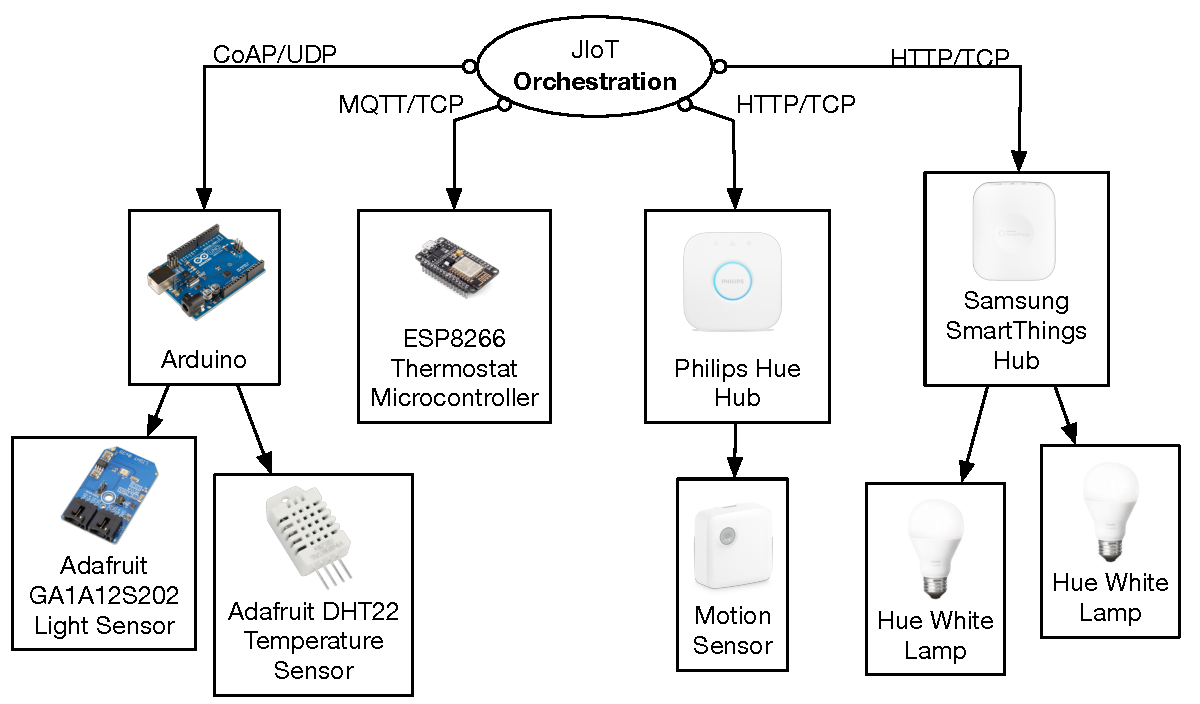
\includegraphics[width=\textwidth]{case_study_overview.pdf}
  \caption{Conceptual overview of the home automation case study.} 
  \label{fig:case_study_overview} \end{figure}

In this section we detail the programming of a JIoT system, focusing on a home
automation case study. We remark that the techniques used in the case study
are not specific of home automation, and can be used in any setting where many
Things based on heterogeneous technologies need to be orchestrated. Notably,
new Things can enter the system at any time. The whole source code of the
system is released under the GPL license\footnote{\url{https://tinyurl.com/ya3vhxyt}}.
We report in \cref{fig:case_study_overview} a schematic overview of the
overall structure of the case study, where Cloud nodes and mid-tier
controllers (represented by the ``JIoT Orchestration'' element in
\cref{fig:case_study_overview}) are programmed in JIoT and orchestrate the
behavior of a number of heterogeneous devices (whose low-level programming is
omitted here):
\begin{itemize}
  \item \emph{Philips Hue Hub}: a hub to control the Philips Hue smart home devices;
  \item \emph{Philips Hue White Lamps}: connected to the hub above;
  \item \emph{Samsung SmartThings Hub}: a hub to control devices following 
  the SmartThings specification~\cite{60};
  \item \emph{Samsung SmartThings Motion Sensor}: connected to the hub above 
  and used as a presence sensor;
  \item \emph{Arduino Uno}: a general-purpose microcontroller;
  \item \emph{Adafruit GA1A12S202 Analog Light Sensor}: connected to the 
  Arduino above;
  \item \emph{Adafruit DHT22 Temperature Sensor}: also connected to the 
  Arduino above;
  \item \emph{ESP8266}: a microcontroller to manage a pre-existing 
  thermostat.
\end{itemize}
This case study has been selected since it involves a heterogeneous
sample of current IoT solutions, to give an account on how JIoT can
manage them.  Concretely, the case study combines commercial
solutions---e.g., the Philips Hue Hub and the Hue White Lamps system
where the Lamps are controlled by the Hub---with custom ones---these
span from sensors directly connected to a board, as it happens for the
Adafruit DHT22 temperature sensor, to solutions that integrate a
pre-existing hardware, like the ESP8266 that manages a pre-existing
thermostat. As illustrated in \cref{fig:case_study_overview}, this
heterogeneity of devices provides for a comprehensive scenario where
we need JIoT programs that use different application and transport
protocols. In particular, Philips and Samsung Hubs communicate with
the orchestrator over HTTP/TCP, the Arduino over MQTT/TCP, and the
ESP8266 over CoAP/UDP.

In the use case we build a simple logic providing two functionalities:
lighting and temperature system control. The lighting system turns on the
lights when the motion sensor detects someone at home and external luminosity
is below some threshold. The temperature control checks the temperature and
turns on the heating system when the temperature is below some threshold. The
threshold has different values depending on whether someone is at home or not.

\begin{figure}[b]
  \centering
  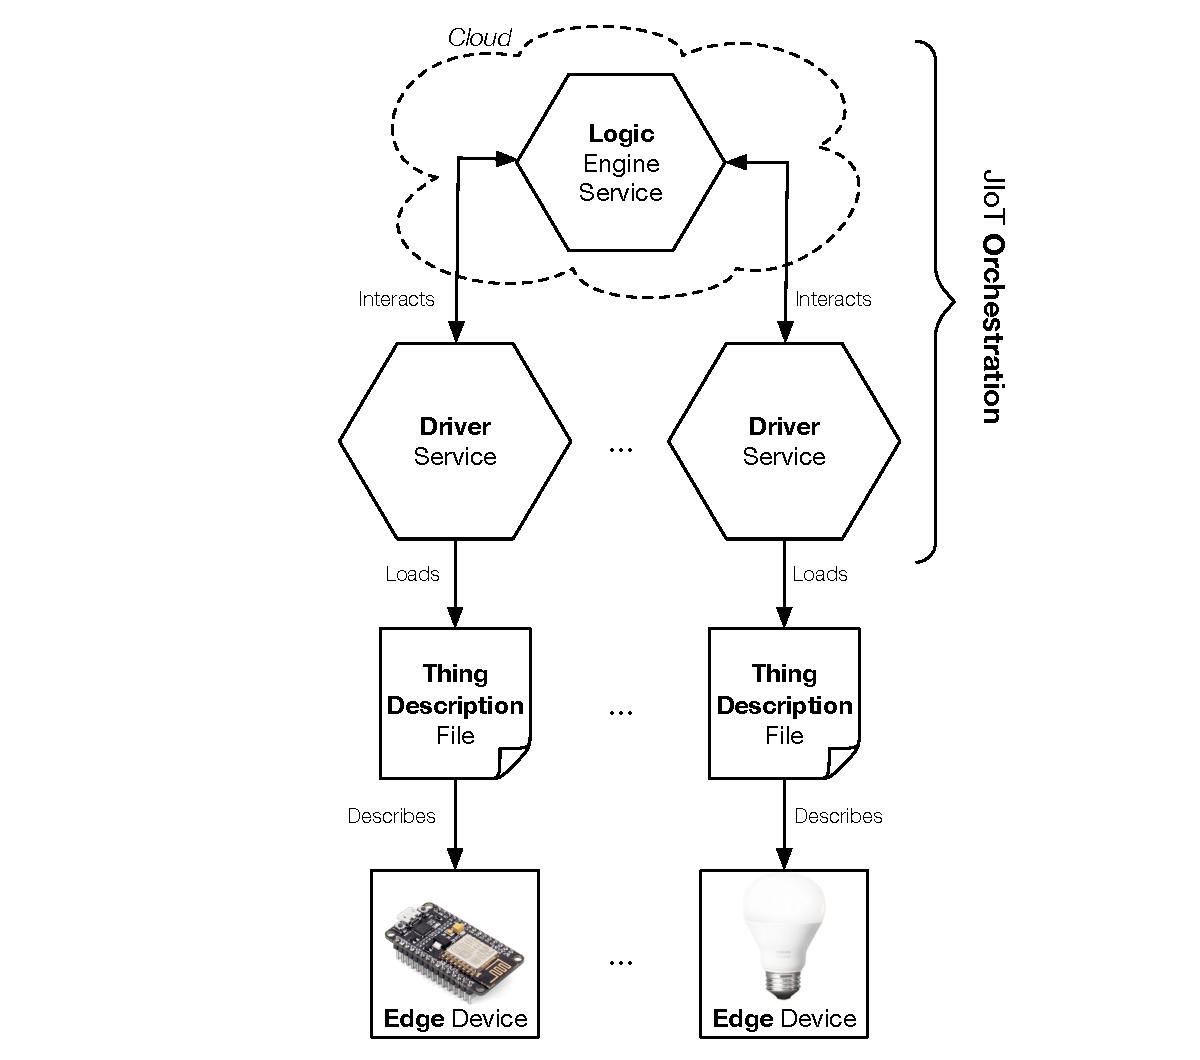
\includegraphics[width=.8\textwidth]{case_study_abstraction.pdf}
  \caption{Scheme of orchestration in the case study.}
  \label{fig:case_study_abstraction}
\end{figure}

\subsection{Structure of the Orchestration}

We now describe the structure of the orchestration in the case study, which is
illustrated in~\cref{fig:case_study_abstraction}.
%
The orchestration is composed of multiple JIoT programs. From top to bottom of
\cref{fig:case_study_abstraction}, the \texttt{LogicEngine} contains the
general logic of system control (i.e., the one that collects data from sensors
and coordinates the execution of actions in the system). Since the
\texttt{LogicEngine} interacts with a multitude of mid-tier devices, its
natural deployment is in the Cloud, where it is possible to scale it according
to the number of managed devices and the load of computation. At the mid-tier
level we have JIoT \texttt{Driver}s. Each \texttt{Driver} interacts with a
specific edge device and it is deployed in a mid-tier machine in the proximity
of the controlled edge device.

\begin{figure}[b]
  \centering
  \begin{lstlisting}[language=json]
{
  "type": "sensor",
  "description": "Thing uses JSON-LD 1.1 serialization",
  "name": "Adafruit DHT22 Temperature Sensor",
  "properties": [
    {
      "temperature": {
        "label": "Celsius"
      }
    }
  ]
}
\end{lstlisting}
\begin{lstlisting}[language=json]
{
  "type": "actuator",
  "description": "Thing uses JSON-LD 1.1 serialization",
  "name": "Philips Hue White Lamp",
  "actions": {
    "toggleLight": {
      "description": "Turn on or off the lamp."
    }
  }
}
\end{lstlisting}
  \caption{Adafruit DHT22 and Philips Hue White Lamp Thing Descriptors}
  \label{fig:sensor_descriptor}
\end{figure}

\subsection{Thing Descriptors}

In the case study, \texttt{Driver}s are statically configured to manage a
single fixed device using a JSON-LD 1.1 (that stands for JSON Linkage Data)
configuration file~\cite{jsonld}. The choice of JSON-LD is not mandatory, but
it has the benefit of following the standard W3C Web of Things~\cite{w3c17}
definition of Thing Description (TD). This makes our \texttt{Driver}s already
compliant with other WoT frameworks, simplifying future integrations with
other WoT systems.

While discussing the full structure of TD is out of the scope of the present
paper, we present in \cref{fig:sensor_descriptor} examples of TDs used in our
case study. In the top half of \cref{fig:sensor_descriptor} we report the TD
for the DHT22 temperature sensor. For each device the JSON-LD file
specifies whether it is a sensor or an actuator (key \lstinline|"type"|) and
provides a textual description (key \lstinline|"description"|) and its name
(key \lstinline|"name"|). Each Thing provides a list of
properties (key \lstinline|"properties"|) that can be read. Each property is
described by the property identifier, \lstinline{"temperature"} in our
example. The property identifier has various sub-elements describing it. In
our example we use just key \lstinline{"label"} to describe the unit of
measure.

JSON-LD configuration files for MQTT and HTTP devices are similar. Also
configuration files for sensors and actuators are similar. As an example, we
reported in the bottom half of \cref{fig:sensor_descriptor} the configuration
file for Philips Hue White Lamps. There the main differences with respect to
the previous TD (top half of \cref{fig:sensor_descriptor}) are:
\begin{itemize}
  \item the \lstinline{"type"} is now {\small\color{color:comment}\texttt{"actuator"}};
  \item the key \lstinline{"actions"} replaces the key \lstinline{"properties"};
  \item the key \lstinline{"description"} is used also to describe the single action.
\end{itemize}

In principle a TD can describe multiple properties belonging to a
group of one or more Things controlled by the same
\texttt{Driver}. For simplicity, here we use one TD for each Thing
and, correspondingly, we have one \texttt{Driver} that controls one
Thing. We also assume that each sensor provides one property.

\subsection{System Deployment}

Deployment-wise, we have a vast choice on which technology stack to use for
the communication between the \texttt{LogicEngine} and the \texttt{Driver}s.
Indeed, since both kinds of programs are developed in JIoT, it is easy to
change their deployment and switch to different technology stacks. Here, we
choose to use the HTTP/TCP stack to make our system compatible with many
existing third-party solutions---currently HTTP/TCP is supported by the
majority of software systems~\cite{richardson2008restful}. However, different
technology stacks fit different purposes. The benefit of JIoT is that
programmers can re-use the same software components adapting their deployment
to the desired communication stacks. For example, if our goal was to minimize
bandwidth usage we could have used the SODEP binary
protocol~\cite{MontesiGZ14} or if we wanted to deploy our system as part of a
Service-Oriented Architecture~\cite{Erl07}, we could have used the SOAP
protocol. While JIoT-to-JIoT deployment is flexible, JIoT-to-Thing
communications are limited by the technology supported by the Thing. Hence, in
our case study each \texttt{Driver} communicates with its Thing using one of
the protocols supported by the latter.


%


\subsection{Components Behavior}

When started, a \code{Driver} loads the TD configuration file of its Thing.
Then it proceeds to register itself to the \code{LogicEngine}. In the
registration, it sends the information retrieved from the TD, enriched with two
additional pieces of information: the address where the Thing can be
contacted---i.e., the \code{Driver} location---and the identifier of the
user to which the Thing belongs. Once registered, the \code{Driver} acts as
a forwarder between the \code{LogicEngine} and the Thing. 

The \code{LogicEngine} runs on the Cloud and manages a number of sensors and
actuators. More precisely the \code{LogicEngine} has one running session for
each user (distinguished according to the user identifier), managing all her
sensors and actuators. Each session is associated with an array of devices
that can be scanned to find the location of \code{device}s with particular
properties and interact with them. As an example, we report at lines 10--27 of
\Cref{lst:logic_example_get} procedure \code{getTemperature} of the
\code{LogicEngine}, which computes the average temperature recorded by the
sensors of one user.
%
\begin{figure}[b]
\begin{lstlisting}[
basicstyle=\footnotesize\ttfamily,
label=lst:logic_example_get,
caption=\code{LogicEngine} \texttt{Driver} \code{outputPort} and \code{getTemperature} procedure.]
interface driverInterface {
  RequestResponse: engineRequest( request )( response )
}

outputPort Driver {
  Protocol: http
  Interfaces: driverInterface
}

define getTemperature {
 sum = 0 ; 
 n = 0 ;
 for ( device in devices ) {
  if( device.<@\textcolor{black}{type}@> == "sensor" && 
    is_defined( device.properties.temperature ) ) {
   Driver.location = device.driverLocation ; 
   request.operationName = "getTemperature" ;
   engineRequest@Driver( request )( response ) ;
   sum = sum + response.deviceResponse ; 
   n++ 
  }
 } ; 
 if( n!=0 ) {
  temperature = sum / n
 } 
}
\end{lstlisting}
\end{figure}
%
Briefly, procedure \code{getTemperature}: 

\begin{itemize}
  \item scans the \lstinline{devices} structure (line 13) containing all
  registered \code{Driver}s;
  \item selects those whose {\small\texttt{type}} is \code{"sensor"} and have
  a property (under the sub-structure \code{properties}) named
  \lstinline{temperature}. Note how Jolie tree-shaped variables ease the
  exploration of structured data; in this case the one sent by the
  \code{Driver}s at registration time (and read from their associated JSON-LD
  file);
  \item it dynamically sets (line 16) the location of \code{outputPort Driver}
  (lines 5-8) to contact the selected \code{Driver};
  \item it sets the request operation to \code{getTemperature} (line 17);
  \item it retrieves the temperature sensed by the Thing controlled by the
  selected \code{Driver}, invoking it through operation \code{engineRequest};
  \item it aggregates the sensed temperature in variable \code{sum} and keeps
  track of the number of requests in variable \code{n} (lines 19--20)
  \item it computes the mean \code{temperature} (lines 23--25).
\end{itemize}
%

The procedures that calculate the mean of the sensed external luminosity and
the one to check the presence of people at home are similar to the one in
\cref{lst:logic_example_get}, except that the searched properties are
\lstinline{light} in the first case, and \lstinline{motion} in the second.

We report in \cref{lst:logic_example_set} one of the procedures managing
actuators, specifically the one used to set the temperature. The main
difference with respect to the logic in \cref{lst:logic_example_get} is that
procedure \code{setTemperature}: 

\begin{itemize}
  \item selects the \lstinline{devices} whose {\small \texttt{type}} is
  \lstinline{"actuator"} (line 3);
  \item sets the request operation to \code{"setTemperature"} and passes the value
  in variable \code{comfortTemperature} as parameter of the request
  (lines 6-7).
\end{itemize}

Note that the operation called on the \code{Driver} is \code{engineRequest}
both in \cref{lst:logic_example_get} and \cref{lst:logic_example_set}. This
enables to extend the \code{LogicEngine} with new procedure definitions that
implement a given goal without requiring to change the interface between the
\code{LogicEngine} and the \code{Driver}s. In turn, a request with the same
\code{operationName} (e.g., \code{"setTemperature"}) triggers different
behaviors in different \code{Driver}s, as each implements the specific logic
of interaction with its associated Thing.
%
\begin{figure}[t]
\begin{lstlisting}[
basicstyle=\footnotesize\ttfamily,
label=lst:logic_example_set,
caption=\code{LogicEngine} setTemperature procedure.]
define setTemperature {
 for ( device in devices ) {
  if( device.<@\textcolor{black}{type}@> == "actuator" && 
    is_defined( device.properties.temperature ) ) {
   Driver.location = device.location ;
   request.operationName = "setTemperature" ;
   request.deviceRequest = comfortTemperature ;
   engineRequest@Driver( request )( response )
  }
 } 
}
\end{lstlisting}
\end{figure}

% They
% would register their devices one-by-one using a suitable security scheme
% (basic, token, api key, etc.). The selection of the security scheme can also
% be specified in the JSON-LD TD. Every time a device for a new user is
% registered, a session of the \code{LogicEngine} managing the devices owned by
% the user is spawned. Thus, new users and new devices can enter the system at
% any time.

\subsection{Cloud Deployment}

We conclude this section by describing the Cloud deployment of the
\code{LogicEngine}, which is containerized using
Docker~\cite{Merkel:2014:DLL:2600239.2600241}. The container is deployed
automatically into an Amazon Web Service cluster via Docker Swarm
manager~\cite{Soppelsa:2017:NDC:3153103}. The \code{LogicEngine} is deployed in
the worker cluster, allowing the manager to balance the load of requests. We
report below the Dockerfile used to deploy the \code{LogicEngine}.
%
\begin{lstlisting}
<@\textcolor{red}{FROM}@> openjdk:alpine

<@\textcolor{red}{RUN}@>  java -jar jiot.jar -jh /usr/lib/jolie/ -jl /usr/bin/
<@\textcolor{red}{ENV}@> JOLIE_HOME /usr/local/lib/jolie

<@\textcolor{red}{ADD}@> logic_engine.ol /home/. 
<@\textcolor{red}{WORKDIR}@> /home
<@\textcolor{red}{RUN}@> jolie logic_engine.ol
\end{lstlisting}
%
At line 1 we declare the starting image for the container, which is the
lightweight Linux Alpine distribution with OpenJDK 8 pre-installed. At lines
3--4 we install the JIoT fork interpreter and we set the environmental
variable \code{JOLIE_HOME} to point to the location of the installed interpreter. Finally, at lines 6--7 we add the source code of the
\code{LogicEngine} in the home directory of the image.
Finally at line 8 we start the execution of the \code{LogicEngine}. 
